\subsection{The current state of ECDAR} %This was written quite fastly ;)
To further illustrate what ECDAR is, and how far its been developed. 
We will go through the tool in this section, a screenshot of which can be found in Figure \ref{fig:ECDAR-gui}. 
The version of ECDAR displayed and described here is ECDAR version 2.3.3 from 2022-09-08 downloaded from \href{https://www.ecdar.net/download/}{www.ecdar.net/download/}.

\begin{figure}[H]
    \centering
    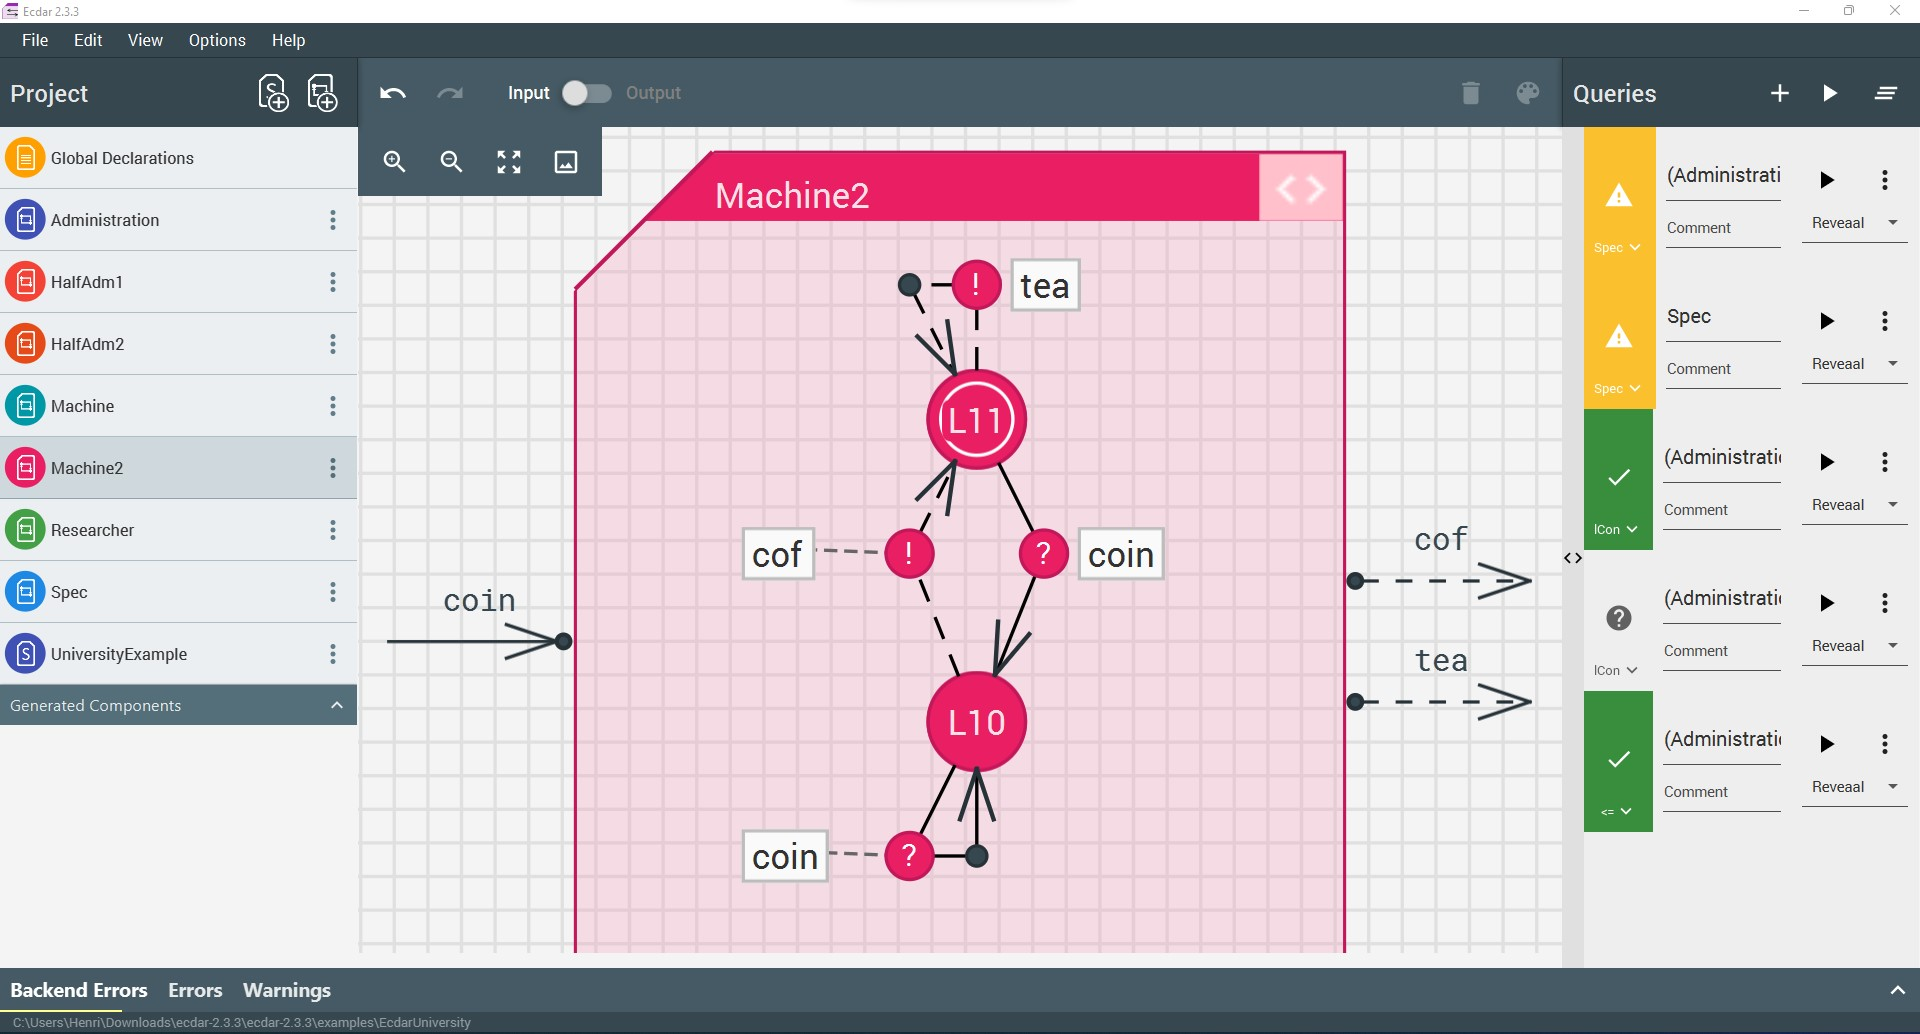
\includegraphics[width=1\textwidth]{common/figures/ecdar-overview.jpg}
    \caption{A screenshot of the ECDAR GUI.}
    \label{fig:ECDAR-gui}
\end{figure}
The top bar of the GUI should be with the five tabs should be pretty self explanatory as it is similar to most "similar programs"/"file editors".
An interesting thing to mention is when opening a project under the \textit{File} tab.
An excisting project is opened by selecting the folder containing two \textit{.json} files: "Queries" and "GlobalDeclarations".
It is not trivial to select a folder to open a project, and neither is it explained in the GUI.
% The top bar of the GUI has five tabs, the leftmost being \textit{File}, this is used to open, save and create new projects. 
% The other tabs are self explanatory.
Positioned right underneath the \textit{Help} tab are the two buttons for creating new models and new specifications under the same project.

The panel on the left contains an overview of the components and specifications. 
In this panel the component \textit{Machine2} is selected which is displayed in the middle of the GUI.
ECDAR allows the user to create a type of automata called \textbf{T}imed \textbf{I}nput \textbf{O}utput \textbf{A}utomata. 
This automaton takes \texttt{coin} as input, since the arrow is solid, and the automaton outputs \texttt{cof} and \texttt{tea}, as shown by the dashed arrows on the left side of the automaton.
Inside the red box the \texttt{L11} location is marked as the start state, which is indicated by the circle.
A solid arrow through a small circle with a question mark represent an output. 
Likewise, if the arrow is dashed and the small circle contains an exclamation mark, it represents an input.
This concludes the possibilities regarding input and output.

Figure \ref{fig:ECDAR-guard} contains an automaton which uses time as well as input and output.
This is done by using a clock, which is represented as the variable y.
\begin{figure}[H]
    \centering
    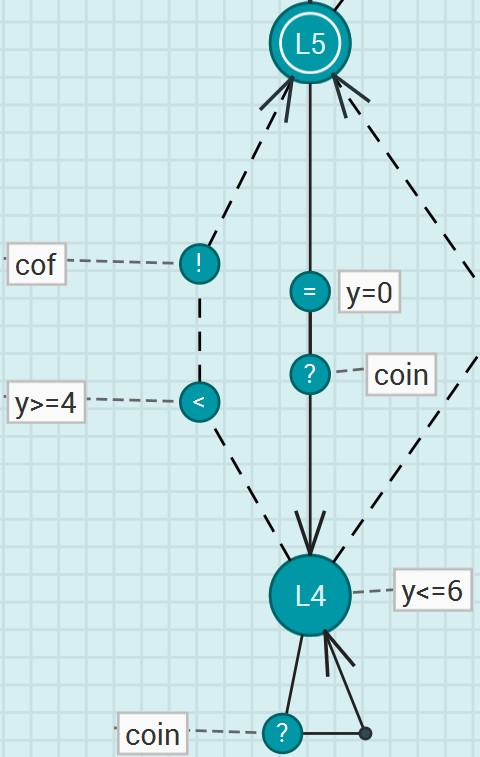
\includegraphics[width=0.3\textwidth]{common/figures/ecdar-guards.jpg}
    \caption{A screenshot of an automaton with a guard and an invariant.}
    \label{fig:ECDAR-guard}
\end{figure}
The transition with the small circle containing the assignment is an \textit{update}, which resets the clock.
The small circle containing a less than sign is a \textit{guard}, which can be thought of as a restriction, which must be satisfied in order to take this action/transition.
Finally the \texttt{L4} location contains an \textit{invariant} \texttt{y<=6}, which must be satisfied. 
In this case it means the automaton cannot be in the location, if the clock value exceeds the value 6.

The rightmost panel displays the queries to be performed. 
Queries are sent to an engine, which can be selected in the drop-down menu, one of which can be seen in the bottom-right corner of Figure \ref{fig:ECDAR-queries-panel}. 
\begin{figure}[H]
    \centering
    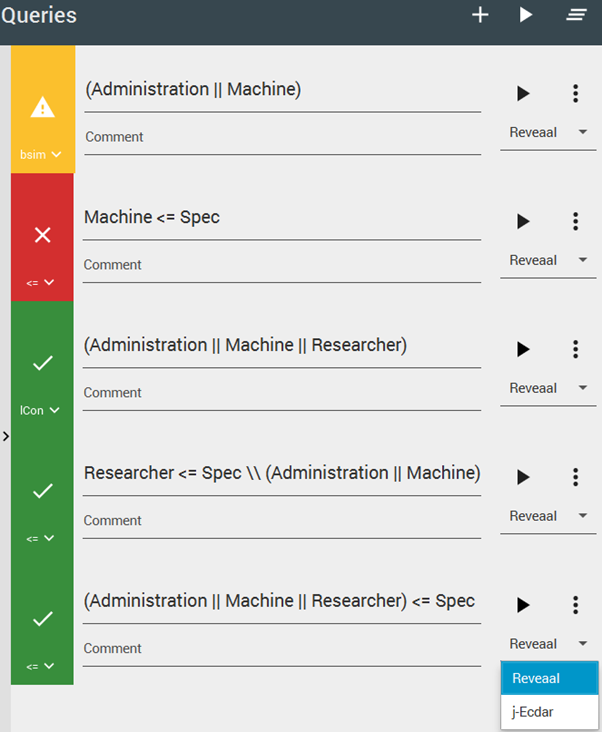
\includegraphics[width=0.6\textwidth]{common/figures/right-panel.png}
    \caption{A screenshot of the right panel of the GUI, which displays the queries.}
    \label{fig:ECDAR-queries-panel}
\end{figure}
To send the queries to be checked, the button with the ``play'' icon must be pressed.
Afterwards the result can be viewed on the left side of the panel in the form of an icon and a color. 
The result of the query in the top of Figure \ref{fig:ECDAR-queries-panel} is an error, which means the engine could not perform the query. 
An error message can be seen by placing the mouse over the icon, which can be used to troubleshoot why this error occurred.
The ``Machine$<=$Spec'' query was performed but the result was false, which means the \texttt{Machine} model does not refine the specification named \texttt{Spec}, which is illustrated by the red color and a cross.
The rest of the queries were performed without errors and all proved true. 
The fields with text use a special syntax to specify a combination of models, operators and specifications to be checked.

\begin{figure}[H]
    \centering
    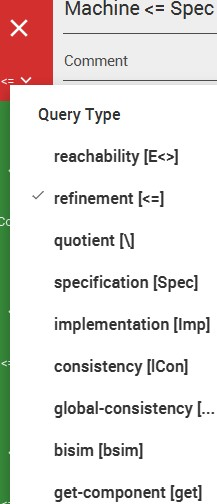
\includegraphics[width=0.25\textwidth]{common/figures/check-type.jpg}
    \caption{A screenshot of drop-down menu with the query types.}
    \label{fig:ECDAR-query-types}
\end{figure}

The type of the query to be performed however is chosen in the drop-down menu underneath the icons. 
The drop-down menu with the types of queries that can be chosen can be seen in figure \ref{fig:ECDAR-query-types}.


